\documentclass[a4paper,12pt]{journal}
\usepackage[dvipsnames, svgnames, x11names]{xcolor} 
\usepackage{amsmath}
\usepackage{amssymb}
\usepackage[margin=2.5cm]{geometry}
\usepackage{graphics}
\usepackage{ulem}
\usepackage{setspace}
\usepackage{listings}
\usepackage{algorithm}  
\usepackage{algpseudocode}  
\usepackage{amsmath}  
\usepackage{xcolor}
\usepackage[greek,english]{babel}
\usepackage{chemformula}
\usepackage{wrapfig}
\usepackage{multirow}
\usepackage{booktabs}
\usepackage{fancyhdr}
\usepackage{pgfplots}
\usepackage{tikz}
\pagestyle{fancy}
\usetikzlibrary{math}
\rmfamily
\fancyhf{}
\fancyfoot[R]{\thepage}
\fancyhead[R]{VG441 Final}
\title{VG441 Final}
\author{Anna Li \\Student ID: 518370910048}
\date{\today}
\lstset{
	columns=fixed,     
	numbers=left,                                        % 在左侧显示行号
	numberstyle=\tiny\color{gray},                       % 设定行号格式
	frame=none,                                          % 不显示背景边框
	backgroundcolor=\color[RGB]{245,245,244},            % 设定背景颜色
	keywordstyle=\color[RGB]{40,40,255},                 % 设定关键字颜色
	numberstyle=\footnotesize\color{darkgray},           
	commentstyle=\it\color[RGB]{0,96,96},                % 设置代码注释的格式
	stringstyle=\ttfamily\slshape\color[RGB]{128,0,0},   % 设置字符串格式
	showstringspaces=false,                              % 不显示字符串中的空格                                        % 设置语言
}
\begin{document}
	\maketitle
	\section*{Problem 1 (Traveling Salesman Problem)}
	\subsection*{Task 1: Run double tree algorithm on paper.}
	1. we draw a graph based on the table, which isFig.1:\\
	\begin{figure}[h]
		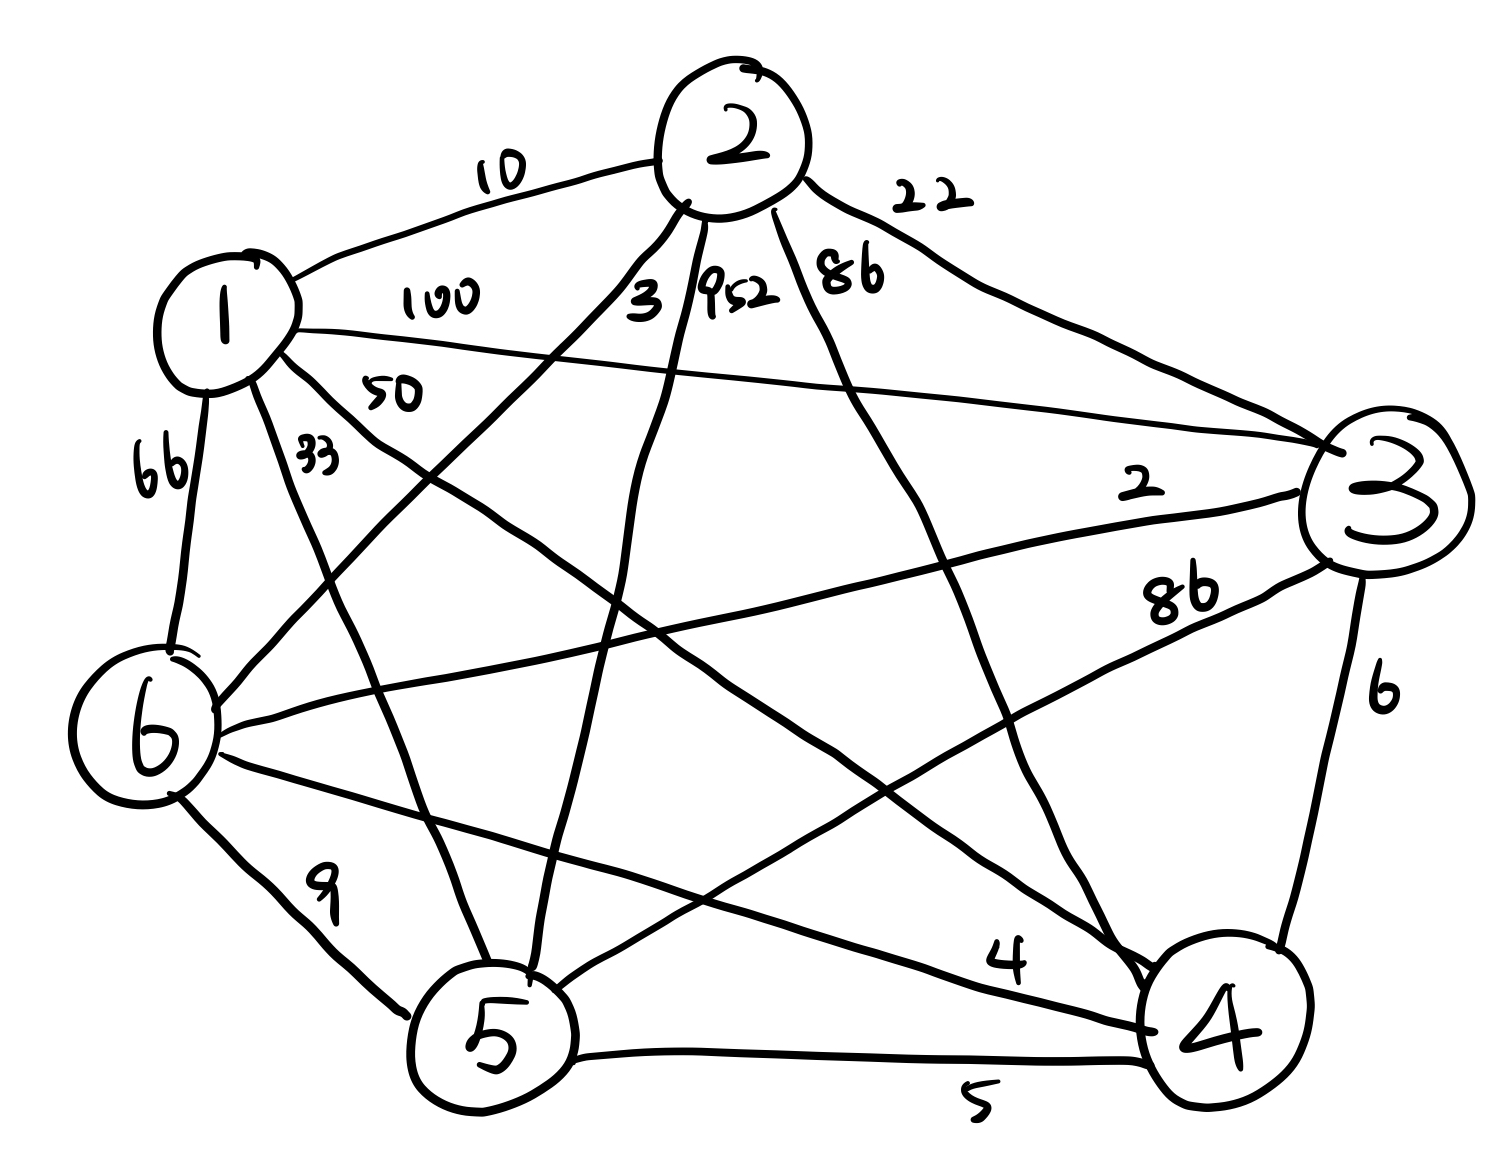
\includegraphics[scale=0.2]{./image/1.jpeg}
		\caption{Original Graph}
	\end{figure}\\
\newpage
	2. We find an MST by kruskal on Fig.2:\\
	\begin{figure}[h]
		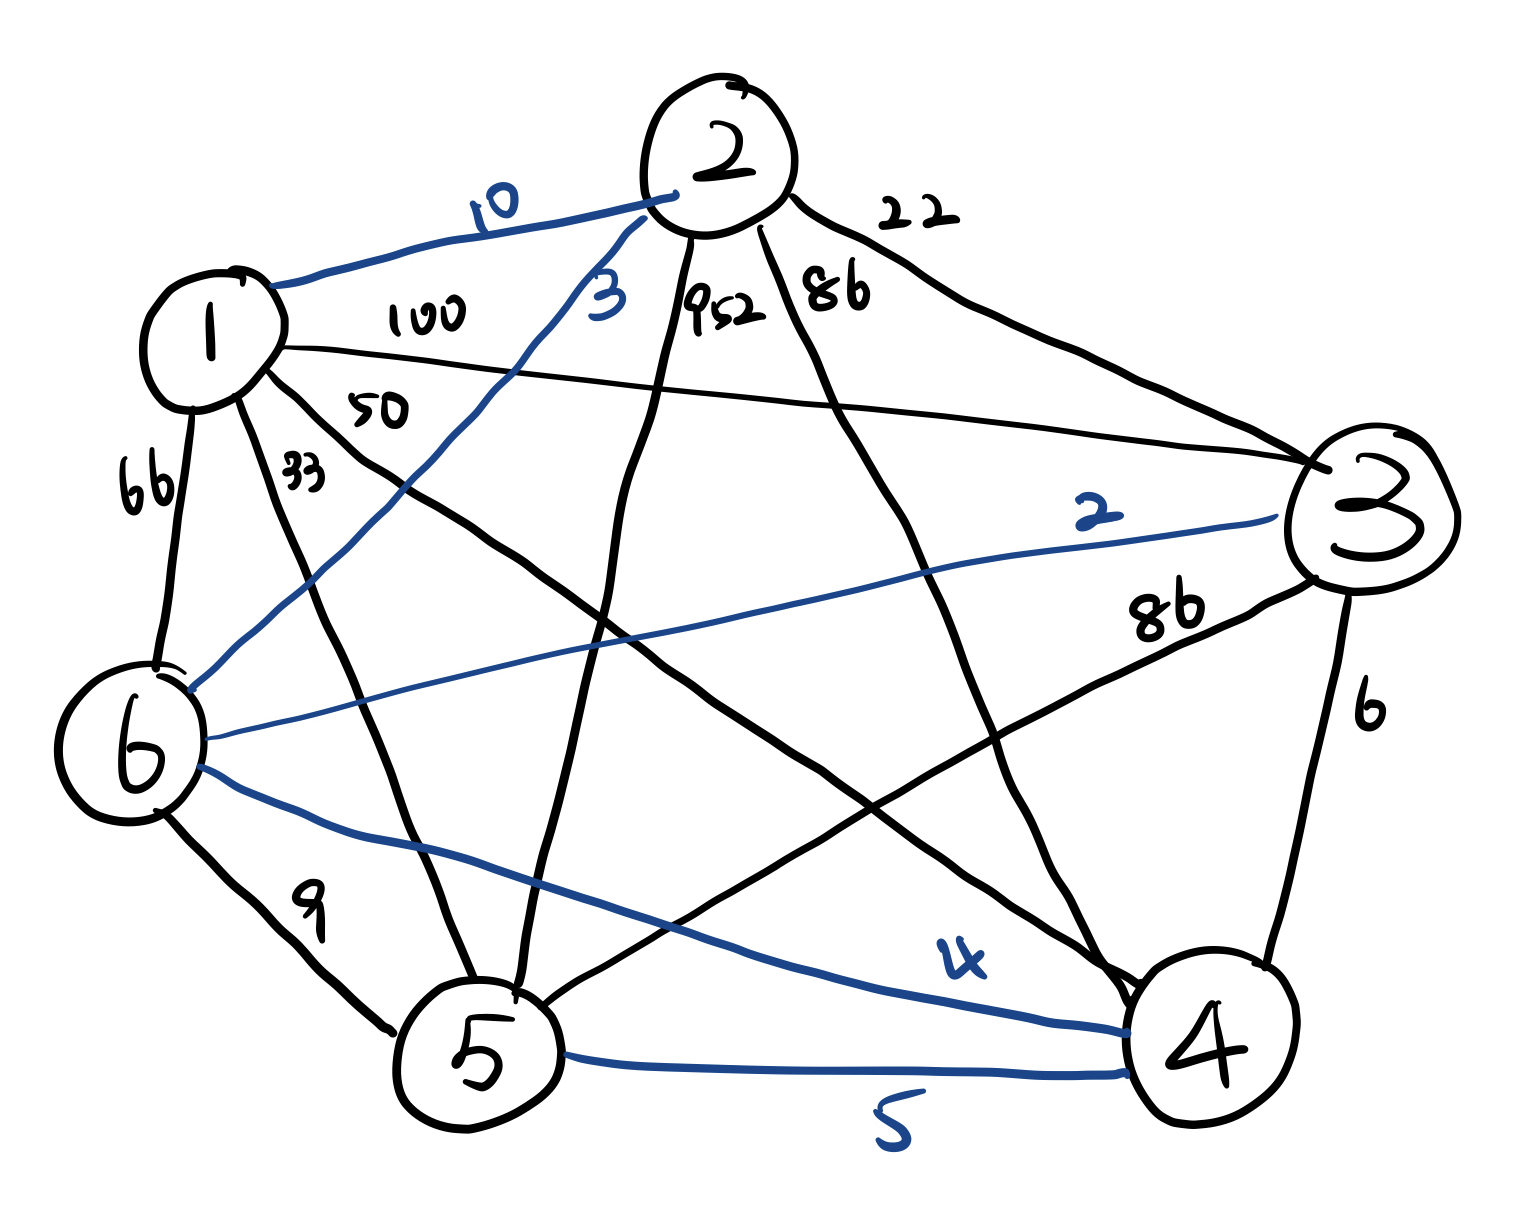
\includegraphics[scale=0.2]{./image/2.jpeg}
		\caption{MST }
	\end{figure}\\
	and if we use (edge, distance ) to express, the MST is:
	(6-2,3),(6-3,2),(6-4,4),(2-1,10),(4-5,5)\\
	3. Double edges of MST and convert it into a tree as fig.3\\
	\begin{figure}[h]
		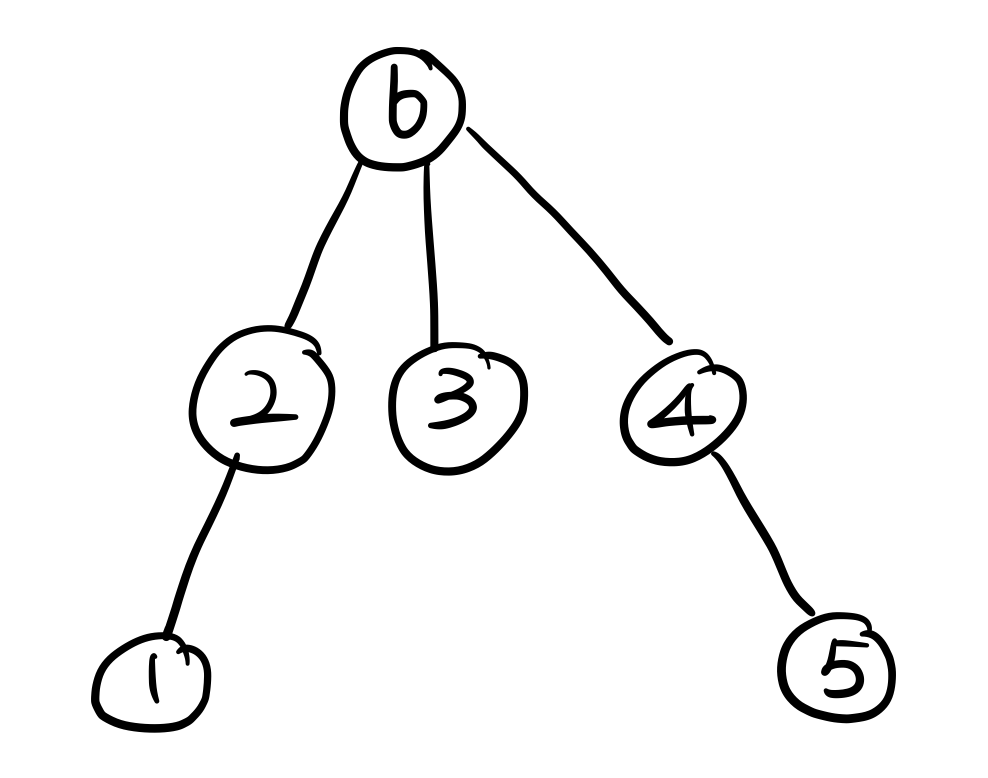
\includegraphics[scale=0.5]{./image/3.png}
		\caption{tree }
	\end{figure}
	According to DFS, we could find a Eulerian path:\\
		$$1\rightarrow2\rightarrow6\rightarrow3\rightarrow6\rightarrow4\rightarrow5\rightarrow4\rightarrow6\rightarrow2\rightarrow1$$
	4. Then we shortcut visited nodes:\\
		$$1\rightarrow2\rightarrow6\rightarrow3\rightarrow4\rightarrow5\rightarrow1$$
		Therefore, the output is $1\rightarrow2\rightarrow6\rightarrow3\rightarrow4\rightarrow5\rightarrow1$ with cost 59
		\subsection*{Task 2: Run Christofides’ algorithm on paper. (Try eyeballing minimum cost matching solution.)}
		For the Christofides’ algorithm, the first 2 steps are same to the double tree algorithm. \\
		3. For the MST we find, the set of odd degree vertices is:\\
		$$\{1,3,5,6\}$$
		Based on this, we find the min-weight-matching K like fig.4:\\
		\begin{figure}[h]
			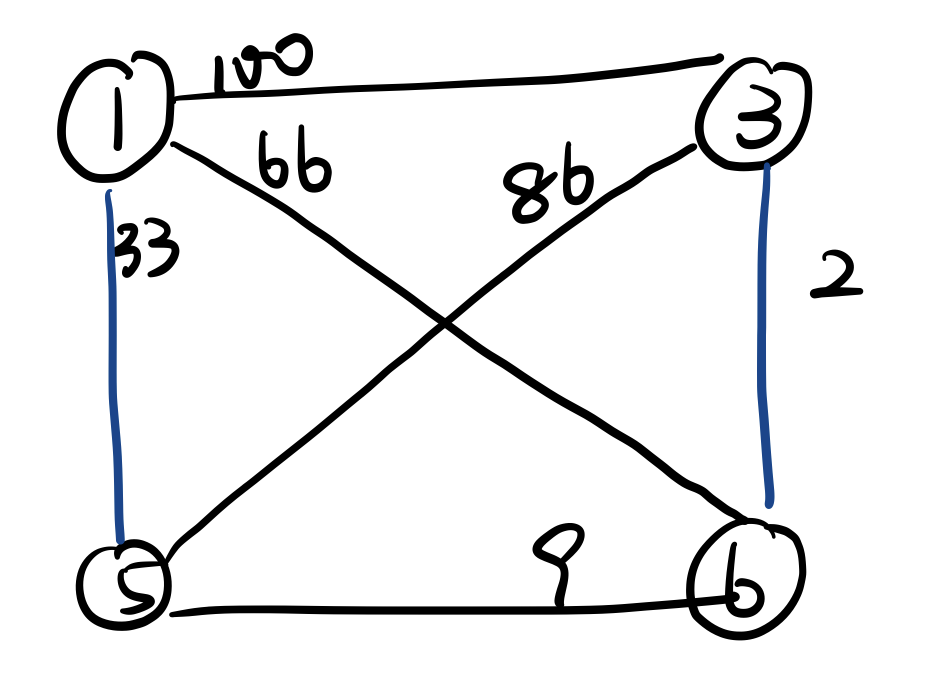
\includegraphics[scale=0.5]{./image/4.png}
			\caption{Min-weight-matching }
		\end{figure}\\
	And we add K to M like fig.5:\\
	\begin{figure}[h]
		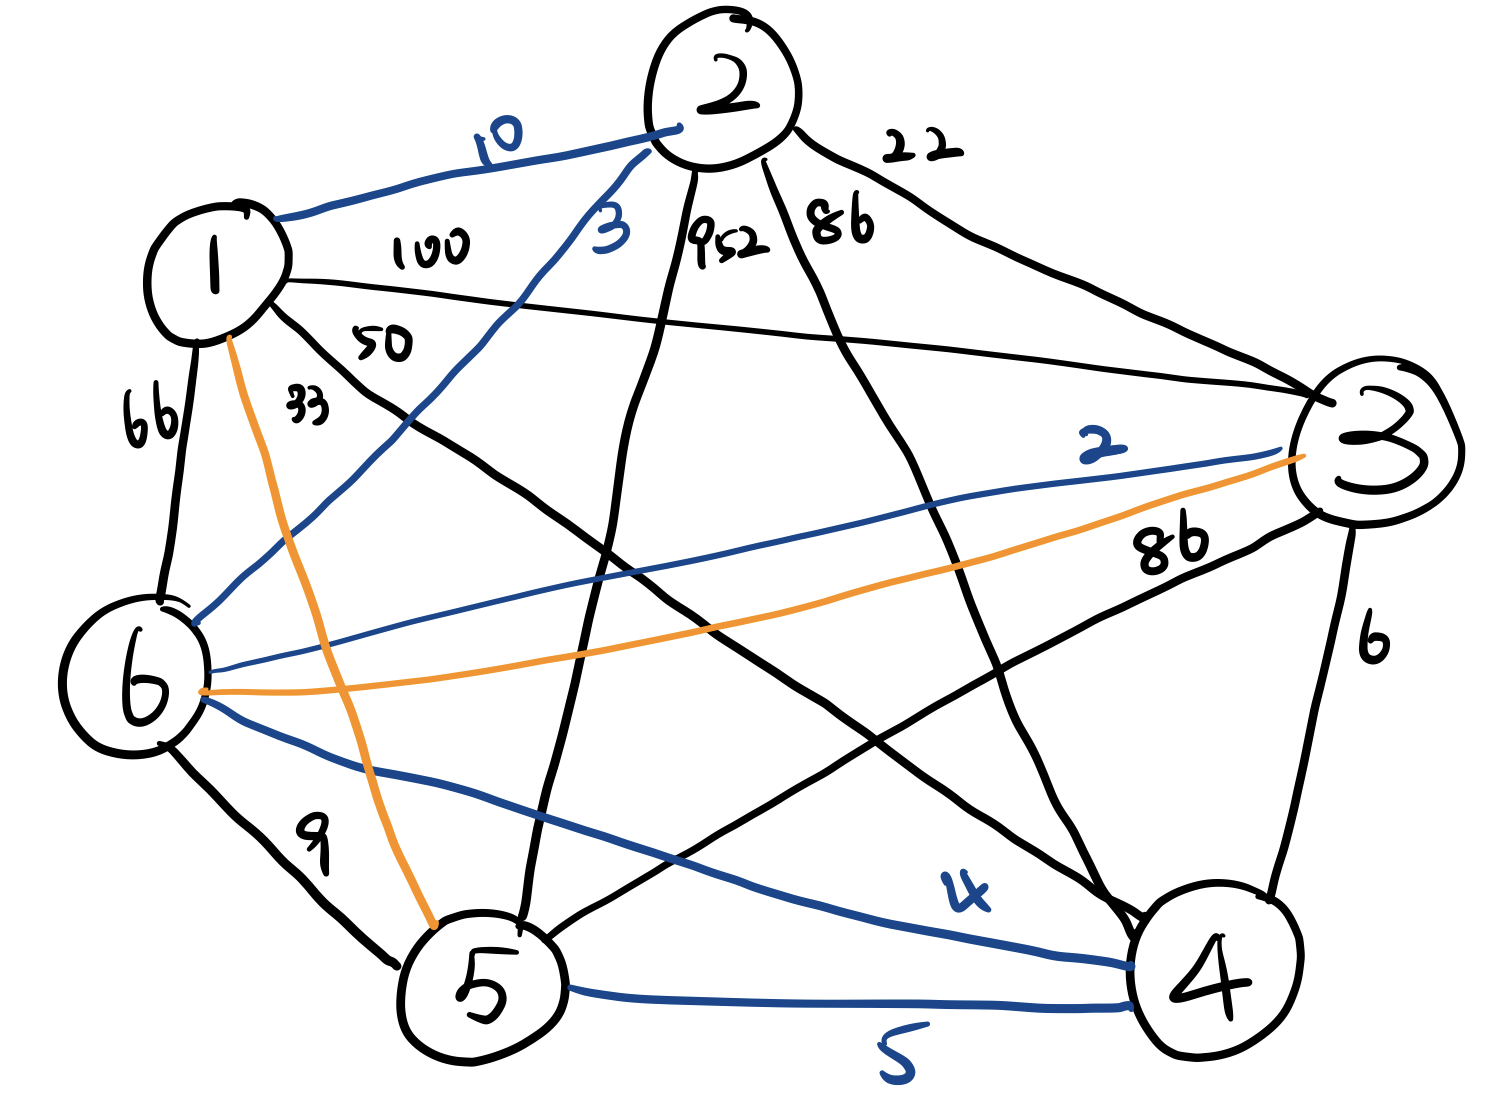
\includegraphics[scale=0.3]{./image/5.png}
		\caption{M+K }
	\end{figure}\\
	4. On the basis of fig.5, we find Eulerian path:
	$$3\rightarrow6\rightarrow2\rightarrow1\rightarrow5\rightarrow4\rightarrow6\rightarrow3$$
	5. Then we shortcutting W:
	$$3\rightarrow6\rightarrow2\rightarrow1\rightarrow5\rightarrow4\rightarrow3$$
	This is the output, and the cost is 59
	\section*{Problem 2 (Knapsack)}
	\subsection*{Task 1: Run the exact dynamic program (ExactKS) on paper to solve this problem.}
	Let T[i,w] be the min-size of  subset $S\subseteq\{1,...,i\}$\\
	Let $v_{max}=6$\\
	$w\in\{0,24\}$
	Therefore, by iteration, we could build a table:
	\begin{center}
		\begin{tabular}{c c c}
			i&w&T\\\hline
			1&0&0\\
			1&4&3\\
			2&0&0\\
			2&4&3\\
			2&8&6\\
			3&0&0\\
			3&4&3\\
			3&6&8\\
			3&8&6\\
			3&10&11\\
			3&14&14\\
			4&0&0\\
			4&4&3\\
			4&5&5\\
			4&6&8\\
			4&8&6\\
			4&9&8\\
			4&10&11\\
			4&11&13\\
			4&13&11\\
			4&14&14\\
			4&15&16\\
			4&19&19\\
		\end{tabular}
	\end{center}
	According to the table, since the bag size is 8, we could know that the best choice is \{4,9,8\}.\\
	The maximum value of w is 9, which means we choose item 1 or 2 and item 4.
	\subsection*{Task 2: Run the simple greedy algorithm (ranking via vi/si) and show that it is not optimal.}
	First, we rank the item with v/s:
	$$\frac{v_1}{s_1}=4/3,\frac{v_2}{s_2}=4/3,\frac{v_4}{s_4}=1,\frac{v_3}{s_3}=3/4$$
	And according to the greedy algorithm, we choose item 1 and item 2, in this way, the value is 8.\\
	Since according to the dynamic program, there is a solution with value of 9, which is greater than 8, therefore, the greedy algorithm is not optimal.
	\section*{Problem 3 (Minimum Cost Set Cover)}
	\subsection*{Task 1: Run this greedy algorithm on paper.}
	In the 1st iteration, 
	$$\text{ratio}_1=\frac{6}{5}\quad\text{ratio}_2=3\quad \text{ratio}_3=1$$
	Therefore, we choose $S_3$ in this iteration\\
	In the 2nd iteration, 
	$$\text{ratio}_1=2\quad\text{ratio}_2=3$$
	Therefore, we choose $S_1$ in this iteration\\
	And in the 3rd iteration, only $S_2$ left, and the ratio is 7.5, so we choose $S_2$\\
	Therefore, we will choose $S_1$,$S_2$,$S_3$ , the total cost is 28.
	\subsection*{Task 2: Is your greedy solution optimal? Can you eyeball a better solution?}
	It is not optimal, because if I choose $S_2$,$S_3$, it could cover all of the set and the cost is only 22, which is smaller than the solution of greedy algorithm.
	\end{document}
